% !TeX program = lualatex
\documentclass[10pt,a4paper]{article}

\usepackage{fontspec}
\setmainfont{Arial}
\setsansfont{Arial}
\usepackage[
  a4paper,
  top=2.54cm,
  bottom=2.54cm,
  left=3cm,
  right=1.5cm
]{geometry}
\usepackage{graphicx}
\usepackage{caption}
\usepackage{microtype}
\usepackage{enumitem}
\usepackage{titlesec}
\usepackage{xcolor}
\usepackage[hidelinks]{hyperref}

\definecolor{sectionblue}{HTML}{1F4E79}
\setlength{\parindent}{0pt}
\setlength{\parskip}{3.2pt}
\setlength{\emergencystretch}{2em}
\pagestyle{empty}
\raggedbottom
\captionsetup{font=normalsize,labelfont=bf,justification=centering,skip=4pt}

\titleformat{\section}
  {\bfseries\color{sectionblue}\fontsize{10.5}{12}\selectfont}
  {}{0pt}{}
\titlespacing*{\section}{0pt}{5pt}{1pt}

\newcommand{\mape}{\mathrm{MAPE}}

\begin{document}

\begin{center}
  {\fontsize{14}{16}\selectfont\bfseries
  MRISystemPhantom Enables Reinforcement-Learning-Based Adaptive $T_1$ Mapping\par}
  \vspace{5pt}
  {\bfseries Arthur Allilaire\textsuperscript{1},
  Andreas Wetscherek\textsuperscript{2},
  Wayne Luk\textsuperscript{1}\par}
  \vspace{3pt}
  {\fontsize{10}{11.5}\selectfont
  \textsuperscript{1}Department of Computing, Imperial College London, London, UK\\
  \textsuperscript{2}Joint Department of Physics, The Institute of Cancer Research and
  The Royal Marsden NHS Foundation Trust, London, UK\par}
\end{center}

\section{Introduction}
Quantitative MRI protocols conventionally fix their acquisition parameters
before scanning so that they remain informative across a wide range of unknown
tissue properties. This robustness can spend limited scan time on redundant
measurements. Adaptive MRI instead uses measurements already acquired to select
the next acquisition, but developing such policies directly on scanner hardware
is costly and provides no exact tissue-parameter ground truth~[2]. We developed
\textit{MRISystemPhantom.jl}, an executable digital twin of the ISMRM/NIST Model
130 system phantom~[3], and used it to test whether reinforcement learning (RL) can
reduce simulated $T_1$-estimation error relative to fixed schedules.

\section{Methods and materials}
\textit{MRISystemPhantom.jl} implements the phantom's water-filled housing,
$T_1$, $T_2$ and proton-density plate geometry, fiducial grid, field-strength
dependent $T_1$/$T_2$ reference values and episode-level tissue randomisation. It returns
standard KomaMRI objects~[1] and supplies the sequence generation, reconstruction,
region-of-interest extraction and signal fitting required for an end-to-end
quantitative simulation.

Each episode acquired noisy two-dimensional inversion-recovery spin-echo images
of five spheres whose $T_1$ values were independently resampled over
$0.04$--$1.9$~s. Complex Gaussian k-space noise produced a mean NEMA MS-1 signal-to-noise
ratio of approximately 17 at the reference acquisition. After each image, the
current $T_1$ values were refitted and a proximal-policy-optimisation agent~[4] chose
the next inversion and repetition times under a 560~s maximum scan budget. The
best policy additionally observed a 12-bin histogram of the inversion times
already executed. Training progressed from an analytic signal model through
cached-water simulations to full Bloch simulation. Frozen policies were tested
over 24 held-out episodes against a policy without acquisition history and two
fixed schedules. The primary endpoint was mean absolute percentage error
($\mape$) in the fitted $T_1$ values, with bootstrap 95\% confidence intervals.

\section{Results}
The TI-history policy achieved a mean $T_1$ $\mape$ of \textbf{2.93\%}
(95\% CI: 2.58--3.30\%), compared with \textbf{6.04\%}
(5.36--6.70\%) for a fixed log-grid schedule under the same maximum budget: a 51.4\% relative
reduction. Its 90th-percentile error was 4.19\%, and 95.8\% of episodes finished
below 5\% error, compared with 7.81\% and 25.0\%, respectively, for the fixed
schedule. Removing the executed-TI histogram increased mean error to 4.16\%
(3.41--4.99\%). The history-aware policy remained below 3.2\% mean error in the
short, intermediate and long realised-$T_1$ bands.

\section{Discussion}
Explicit acquisition history improved the policy despite a similar number of
measurements, indicating that the running $T_1$ estimates alone did not fully
describe which parts of inversion-time space had already been sampled. The
digital phantom made this comparison reproducible across known, continuously
varying tissue properties. The positive result is limited to a five-sphere,
simulator-only proof of concept with one training seed and 24 evaluation
episodes; the policy did not outperform fixed coverage on the complete
14-sphere plate.

\section{Conclusion}
\textit{MRISystemPhantom.jl} provides a reusable quantitative testbed for
adaptive MRI development. Within a bounded simulated $T_1$-mapping task, an RL
policy that remembered its previous inversion times substantially outperformed
fixed acquisition schedules.

\newpage

\begin{figure}[!ht]
  \centering
  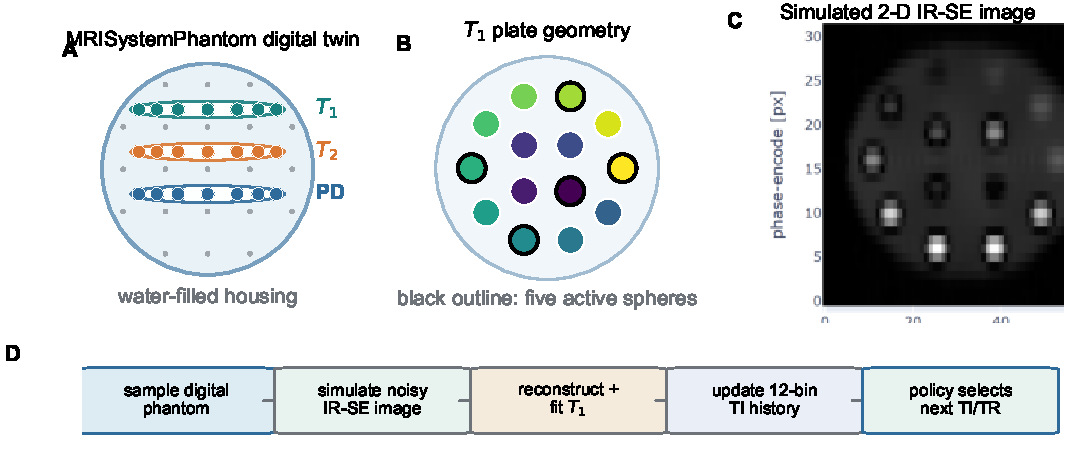
\includegraphics[width=\linewidth]{figures/method_overview.pdf}
  \caption{\textbf{MRISystemPhantom and the adaptive acquisition method.}
  \textbf{A:} Configurable digital representation of the Model 130 phantom.
  \textbf{B:} $T_1$-plate geometry; black outlines identify the five active
  positions whose values are resampled each episode. \textbf{C:} Example Bloch-simulated IR-SE
  reconstruction. \textbf{D:} Closed-loop experiment in which the policy uses
  fitted $T_1$ values and an executed-TI histogram to select the next timing.}
\end{figure}

\vspace{3pt}

\begin{figure}[!ht]
  \centering
  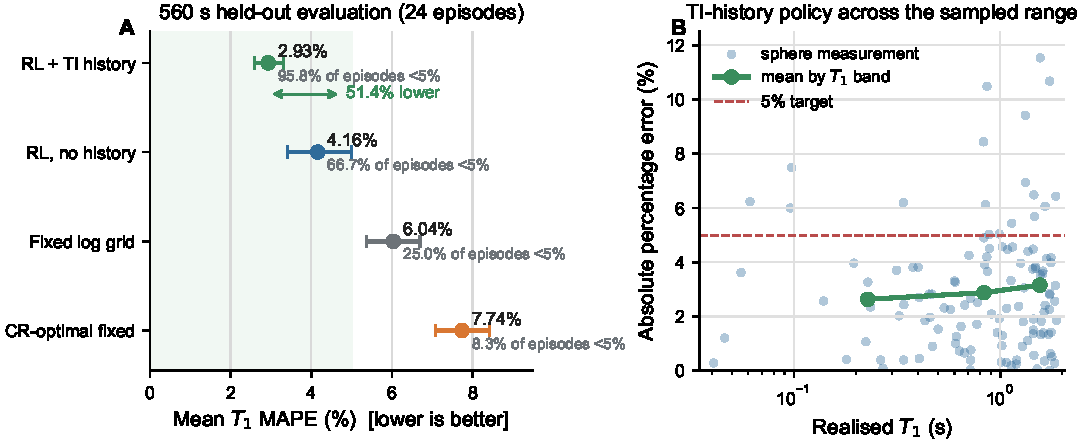
\includegraphics[width=\linewidth]{figures/heldout_results.pdf}
  \caption{\textbf{Five-sphere held-out result.}
  \textbf{A:} Mean fitted-$T_1$ error with 95\% confidence intervals; percentages
  beneath each point give the fraction of episodes below 5\% error.
  \textbf{B:} Absolute error for all 120 held-out sphere measurements, with means
  over short, intermediate and long realised-$T_1$ bands.}
\end{figure}

\vfill
\section{References}
\begin{enumerate}[leftmargin=*,label=\arabic*.,itemsep=0pt,topsep=1pt,parsep=0pt]
  \item Castillo-Passi et al. \textit{Magn Reson Med}. 2023;90:329--342.
  \item Beracha et al. \textit{Magn Reson Med}. 2023;90:839--851.
  \item Russek et al. \textit{Proc Int Soc Magn Reson Med}. 2020;3384.
  \item Schulman et al. \textit{arXiv}. 2017;1707.06347.
\end{enumerate}

\section{Acknowledgements}
This work formed part of Arthur Allilaire's BEng final-year project at Imperial
College London.

\end{document}
